% !TeX program = xelatex
\documentclass[a4paper,10pt]{article}

% ============================================================================
% សន្លឹកកិច្ចការសិស្សបំពេញចន្លោះ ស-ខ្មៅ និងប្លង់ក្ដារខៀន/ចម្លើយគ្រូ (គ្មាន LCD / គ្មានកន្ត្រៃ)
% មេរៀនទី២ (៦.)៖ ពហុគុណរួមតូចបំផុត (PPCM ឬ LCM) និងសំយោគមេរៀនទី២ — ត្រូវគ្នា ១០០% នឹង LS_Plan_DIV26.tex
% ============================================================================
\usepackage[a4paper, left=1.0cm, right=1.0cm, top=0.75cm, bottom=1.00cm, footskip=0.52cm]{geometry}
\usepackage{amsmath}
\usepackage{unicode-math}
\usepackage{fontspec}
\usepackage{array, colortbl}
\usepackage[table]{xcolor}
\usepackage{enumitem}
\usepackage{pifont}
\usepackage{fancyhdr}
\usepackage{lastpage}
\usepackage{tikz}
\usepackage[most]{tcolorbox}
\usetikzlibrary{calc, arrows.meta, decorations.pathreplacing, patterns, positioning, babel}

\makeatletter
\let\@expl@@@mark@update@singlecol@structures@@\relax
\makeatother

\providecommand{\NGSFindFonts}{%
  \IfFileExists{C:/Windows/Fonts/cambria.ttc}{%
    \def\NGSSysPath{C:/Windows/Fonts/}%
    \def\NGSUserPath{C:/Users/KIT/AppData/Local/Microsoft/Windows/Fonts/}%
  }{%
    \IfFileExists{./fonts/KhmerOSsiemreap.ttf}{\def\NGSSysPath{./fonts/}\def\NGSUserPath{./fonts/}}{%
    \IfFileExists{../fonts/KhmerOSsiemreap.ttf}{\def\NGSSysPath{../fonts/}\def\NGSUserPath{../fonts/}}{%
    \IfFileExists{../../fonts/KhmerOSsiemreap.ttf}{\def\NGSSysPath{../../fonts/}\def\NGSUserPath{../../fonts/}}{%
    \IfFileExists{../../../fonts/KhmerOSsiemreap.ttf}{\def\NGSSysPath{../../../fonts/}\def\NGSUserPath{../../../fonts/}}{%
    \IfFileExists{../../../../fonts/KhmerOSsiemreap.ttf}{\def\NGSSysPath{../../../../fonts/}\def\NGSUserPath{../../../../fonts/}}{%
    \IfFileExists{../../../../../fonts/KhmerOSsiemreap.ttf}{\def\NGSSysPath{../../../../../fonts/}\def\NGSUserPath{../../../../../fonts/}}{%
    \IfFileExists{../../../../../../fonts/KhmerOSsiemreap.ttf}{\def\NGSSysPath{../../../../../../fonts/}\def\NGSUserPath{../../../../../../fonts/}}{%
      \def\NGSSysPath{../../../../../../../fonts/}\def\NGSUserPath{../../../../../../../fonts/}%
    }}}}}}}%
  }%
}
\NGSFindFonts

\setmathfont[Path={\NGSSysPath}, FontIndex=1, Scale=1.02]{cambria.ttc}
\defaultfontfeatures{Ligatures=TeX}

\setmainfont[
  Path={\NGSUserPath}, Extension=.ttf, Script=Khmer,
  BoldFont={KhmerOSsiemreap}, BoldFeatures={FakeBold=1.8},
  ItalicFont={KhmerOSsiemreap}, ItalicFeatures={FakeSlant=0.25},
  BoldItalicFont={KhmerOSsiemreap}, BoldItalicFeatures={FakeBold=1.8, FakeSlant=0.25}
]{KhmerOSsiemreap}

\newfontfamily\muol[Path={\NGSUserPath}, Extension=.ttf, Script=Khmer]{KhmerOSmuollight}
\newfontfamily\TimesEn[Path={\NGSSysPath}, Extension=.ttf, BoldFont={timesbd}, ItalicFont={timesi}, BoldItalicFont={timesbi}]{times}
\newfontfamily\CalibriFont[Path={\NGSSysPath}, Extension=.ttf]{calibri}

\XeTeXlinebreaklocale "km"
\XeTeXlinebreakskip = 0pt plus 1pt minus 0.1pt

\definecolor{panelgray}{gray}{0.94}
\definecolor{headgray}{gray}{0.85}

\pagestyle{fancy}
\fancyhf{}
\renewcommand{\headrulewidth}{0pt}
\fancyfoot[L]{\fontsize{7.4pt}{9.5pt}\selectfont អនុវិទ្យាល័យព្រះក្រសាំង \en{|} គ្រូ៖ ហុក ប៊ុនថែន \en{|} មេរៀនទី២ (៦.) ពហុគុណរួមតូចបំផុត (\en{PPCM}) \en{|} ថ្ងៃពុធ ទី១៨ ខែវិច្ឆិកា ឆ្នាំ២០២៦}
\fancyfoot[R]{\fontsize{7.8pt}{10pt}\selectfont ទំព័រ \en{\thepage\ / \pageref{LastPage}}}

\setlength{\parindent}{0pt}
\setlength{\parskip}{0pt}
\setlength{\tabcolsep}{4pt}
\newcolumntype{L}[1]{>{\raggedright\arraybackslash}p{#1}}
\newcolumntype{C}[1]{>{\centering\arraybackslash}p{#1}}

\newcommand{\en}[1]{{\TimesEn #1}}
\newcommand{\enbf}[1]{{\TimesEn\bfseries #1}}
\newcommand{\unit}[1]{\,\text{\en{#1}}}
\newcommand{\cnum}[1]{\mbox{\fontsize{10pt}{12pt}\selectfont\ding{\numexpr181+#1\relax}}}
\newcommand{\chkbox}{\tikz[baseline=-0.15ex]\draw[black, line width=0.85pt, fill=white] (0,0) rectangle (0.24cm,0.24cm);}
\newcommand{\ansbox}[1][1.75cm]{\,\tikz[baseline=-0.65ex]\draw[black, line width=0.65pt, fill=white] (0,0) rectangle (#1, 0.42cm);\,}
\newcommand{\dotline}[1][2.2cm]{\makebox[#1]{\dotfill}}

\newcommand{\pagebanner}[2]{%
  \begin{tcolorbox}[
    enhanced, sharp corners, colback=headgray, colframe=black,
    boxrule=1.05pt, boxsep=1pt, top=2.5pt, bottom=2.5pt, left=6pt, right=6pt,
    after skip=3.5pt
  ]
    {\muol\fontsize{9.0pt}{13.2pt}\selectfont #1}\hfill{\fontsize{8.0pt}{11.2pt}\selectfont\textbf{#2}}
  \end{tcolorbox}%
}

\newcommand{\secstrip}[2]{%
  \vspace{3pt}%
  \begin{tcolorbox}[
    enhanced, sharp corners, colback=panelgray, colframe=black,
    boxrule=0.8pt, boxsep=0.8pt, top=2pt, bottom=2pt, left=5pt, right=5pt,
    after skip=3pt
  ]
    {\muol\fontsize{8.5pt}{12.2pt}\selectfont #1}\hfill{\fontsize{7.8pt}{10.8pt}\selectfont\textit{#2}}
  \end{tcolorbox}%
}

\begin{document}
\fontsize{9.5pt}{14.5pt}\selectfont

% ============================================================================
% ទំព័រទី ១៖ សន្លឹកកិច្ចការសិស្ស (ផ្នែកមុខ៖ E1 -> E2 -> E3)
% ============================================================================
\pagebanner{សន្លឹកកិច្ចការសិស្ស \enbf{(}៦\enbf{.} ពហុគុណរួមតូចបំផុត \enbf{PPCM} និងសំយោគមេរៀនទី២\enbf{)} \enbf{--} ផ្នែកមុខ}{ថ្នាក់ទី៧ \en{|} សៀវភៅគោល ទំ.២២--២៣}

\begin{tcolorbox}[
  enhanced, sharp corners, colback=white, colframe=black,
  boxrule=0.8pt, boxsep=1.5pt, top=3.5pt, bottom=3.5pt, left=5pt, right=5pt,
  after skip=4pt
]
  \fontsize{9.0pt}{13.0pt}\selectfont
  \textbf{ឈ្មោះសិស្ស៖} \dotline[4.3cm] \quad
  \textbf{សមាជិកក្រុម៖} \dotline[4.3cm] \quad
  \textbf{ថ្នាក់ទី៖} ៧\dotline[0.9cm] \quad
  \textbf{ក្រុមទី៖} \dotline[1.0cm]
\end{tcolorbox}

% --- E1 Engage ---
\secstrip{ផ្នែកទី ១ \enbf{(E1 - Engage)} ៖ បេសកកម្មអន្ទាក់ពាក្យ «តូចបំផុត» ក្នុង $\operatorname{PPCM}(6, 8)$}{រយៈពេល ៣ នាទី (គូស \ding{51} ក្នុង \chkbox)}

\begin{tcolorbox}[
  enhanced, sharp corners, colback=white, colframe=black,
  boxrule=0.8pt, boxsep=2pt, top=4pt, bottom=4pt, left=6pt, right=6pt
]
  គេដឹងថា $6 = 2 \times 3$ និង $8 = 2^3$ ។ គេចង់រក\textbf{ពហុគុណរួមតូចបំផុត} $\operatorname{PPCM}(6, 8)$៖\\[2.5pt]
  $\bullet$ \chkbox\ \textbf{សិស្ស ក៖} «ព្រោះរកពហុគុណរួម\textbf{តូចបំផុត} ត្រូវយកតែកត្តារួមនិទស្សន្តតូចជាងគេ គឺ $2$!»\\[2pt]
  $\bullet$ \chkbox\ \textbf{សិស្ស ខ៖} «$2$ ចែកមិនដាច់នឹង $6$ ឬ $8$ ទេ! ត្រូវយកកត្តារួមនិទស្សន្តធំ ($2^3$) គុណនឹងកត្តាមិនរួម ($3$) បាន $2^3 \times 3 = 24$ ទើបចែកដាច់ទាំងពីរ!»
\end{tcolorbox}

\vfill

% --- E2 Explore ---
\secstrip{ផ្នែកទី ២ \enbf{(E2 - Explore)} ៖ ប្រអប់ជួរឈររក $\operatorname{PPCM}$ និងប្រៀបធៀបនឹង $\operatorname{PGCD}$ (ទំ.២២--២៣)}{រយៈពេល ១១ នាទី}

\textbf{សកម្មភាព ១ (\en{E2-A} — ៥.៥ នាទី)៖ រក $\operatorname{PPCM}(6, 8)$ តាមវិធីទាំងពីរ (ឧទាហរណ៍ 1 ទំ.២២)}

\begin{tcolorbox}[
  enhanced, sharp corners, colback=white, colframe=black,
  boxrule=0.8pt, boxsep=2.5pt, top=4pt, bottom=4pt, left=6pt, right=6pt
]
  \begin{minipage}[t]{0.48\textwidth}
    \textbf{១) វិធីទី 1៖ រាយពហុគុណមិនសូន្យ}\\[2.5pt]
    $\bullet$ ពហុគុណនៃ $6$: $6, 12, 18,$ \dotline[0.7cm], $30, 36, 42,$ \dotline[0.7cm], $\dots$\\[2.5pt]
    $\bullet$ ពហុគុណនៃ $8$: $8, 16,$ \dotline[0.7cm], $32, 40,$ \dotline[0.7cm], $56, \dots$\\[2.5pt]
    $\bullet$ ពហុគុណរួមតូចបំផុត៖ $\operatorname{PPCM}(6, 8) =$ \ansbox[1.3cm]
  \end{minipage}\hfill
  \vrule width 0.6pt\hfill
  \begin{minipage}[t]{0.48\textwidth}
    \textbf{២) វិធីទី 2៖ តម្រឹមជួរឈរកត្តាបឋម (ទំ.២២)}\\[2.5pt]
    \hspace*{0.4cm}$6 = \;\;2\;\; \times 3$\\[2pt]
    \hspace*{0.4cm}$8 = \;\;2^3$\\[2.5pt]
    ទម្លាក់៖ $\operatorname{PPCM}(6, 8) =$ \dotline[0.8cm] $\times$ \dotline[0.7cm] $=$ \ansbox[1.3cm]
  \end{minipage}
\end{tcolorbox}

\vspace{4pt}
\textbf{សកម្មភាព ២ (\en{E2-B} — ៥.៥ នាទី)៖ ចំនួនបីតួ និងការប្រៀបធៀបផ្ទាល់ជាមួយ $\operatorname{PGCD}$ (ឧទាហរណ៍ 2 ទំ.២២--២៣)}

\begin{tcolorbox}[
  enhanced, sharp corners, colback=white, colframe=black,
  boxrule=0.8pt, boxsep=2.5pt, top=4.5pt, bottom=4.5pt, left=6pt, right=6pt
]
  \begin{minipage}[t]{0.50\textwidth}
    \textbf{១) ឧទាហរណ៍ 2៖ រក $\operatorname{PPCM}(18, 24, 36)$}\\[2pt]
    \hspace*{0.2cm}$18 = 2\phantom{^3} \times 3^2$\\
    \hspace*{0.2cm}$24 = 2^3 \times 3\phantom{^2}$\\
    \hspace*{0.2cm}$36 = 2^2 \times 3^2$\\[2.5pt]
    $\operatorname{PPCM}(18, 24, 36) =$ \dotline[0.8cm] $\times$ \dotline[0.8cm] $=$ \ansbox[1.3cm]
  \end{minipage}\hfill
  \vrule width 0.6pt\hfill
  \begin{minipage}[t]{0.46\textwidth}
    \textbf{២) ប្រៀបធៀបឆ្លាស់គ្នាលើ $(18, 24, 36)$ និង $(6, 8)$៖}\\[2pt]
    $\bullet$ ឯ $\operatorname{PGCD}(18, 24, 36) =$ \dotline[0.7cm] $\times$ \dotline[0.7cm] $=$ \ansbox[1.1cm]\\[2.5pt]
    $\bullet$ លើ $(6, 8)$៖ $\operatorname{PGCD}\times\operatorname{PPCM} = 2\times 24 =$ \dotline[0.9cm]\\[2pt]
    \hspace*{0.2cm}ហើយ $6 \times 8 =$ \dotline[0.9cm] (ស្មើគ្នាបេះបិទ!)
  \end{minipage}
\end{tcolorbox}

\vfill

% --- E3 Explain ---
\secstrip{ផ្នែកទី ៣ \enbf{(E3 - Explain)} ៖ វិធានទូទៅ និងតារាងញែកលក្ខណៈ \enbf{PGCD} ទល់នឹង \enbf{PPCM}}{រយៈពេល ៦ នាទី}

\begin{tcolorbox}[
  enhanced, sharp corners, colback=white, colframe=black,
  boxrule=0.85pt, boxsep=2.5pt, top=4pt, bottom=4pt, left=6pt, right=6pt
]
  $\bullet$ \textbf{ជាទូទៅ (ទំ.២៣)៖} ដើម្បីរក $\operatorname{PPCM}$ នៃពីរឬច្រើនចំនួន គេបំបែកចំនួននីមួយៗជាផលគុណកត្តាបឋម រួចគុណ\textbf{កត្តារួមដែលមាននិទស្សន្ត\dotline[1.8cm]} ជាមួយនឹង\textbf{កត្តា\dotline[1.8cm]} ដែលមានក្នុងចំនួនទាំងនោះ ។\\[3pt]
  \tikz\draw[black, dashed, line width=0.5pt] (0,0) -- (18.4cm,0);\\[3pt]
  \fontsize{8.6pt}{12.6pt}\selectfont
  \textbf{ធនាគារហេតុផល (\en{Warrant Bank})៖} \quad
  \cnum{1} $\operatorname{PPCM}(a,b) \ge \max(a,b)$ (ចែកដាច់នឹងទាំង $a$ និង $b$) \quad
  \cnum{2} $\operatorname{PPCM} =$ កត្តារួម (និទស្សន្តធំ) $\times$ កត្តាមិនរួម\\
  \cnum{3} កាត់បំបែក/ចែកស្មើ $\to \operatorname{PGCD}$ $\;\mid\;$ រៀបផ្គុំ/ជួបដំណាលគ្នា $\to \operatorname{PPCM}$ \quad
  \cnum{4} $N$ ចែកនឹង $x$ សល់ $r \implies (N - r)$ ចែកដាច់នឹង $x$ ($x > r$)
\end{tcolorbox}

% ============================================================================
% ទំព័រទី ២៖ សន្លឹកកិច្ចការសិស្ស (ផ្នែកខាងខ្នង៖ E4 -> E5 -> កិច្ចការផ្ទះ)
% ============================================================================
\clearpage
\pagebanner{សន្លឹកកិច្ចការសិស្ស \enbf{(}៦\enbf{.} ពហុគុណរួមតូចបំផុត \enbf{PPCM} និងសំយោគមេរៀនទី២\enbf{)} \enbf{--} ផ្នែកខាងខ្នង}{ថ្នាក់ទី៧ \en{|} សៀវភៅគោល ទំ.២៣--២៤}

% --- E4 Elaborate ---
\secstrip{ផ្នែកទី ៤ \enbf{(E4 - Elaborate)} ៖ លំហាត់គំរូតាមសៀវភៅគោល ទំ.២៣ (រៀបសន្លឹកប័ណ្ណជាការេ)}{រយៈពេល ១០ នាទី}

\begin{tcolorbox}[
  enhanced, sharp corners, colback=white, colframe=black,
  boxrule=0.8pt, boxsep=2.5pt, top=4.5pt, bottom=4.5pt, left=6pt, right=6pt
]
  \textbf{ប្រធាន (ទំ.២៣)៖} គេរៀបសន្លឹកប័ណ្ណតូចៗជារាងចតុកោណកែងមានបណ្ដោយ $12\unit{cm}$ និងទទឹង $9\unit{cm}$ តាមទិសដៅដូចគ្នាដើម្បីបង្កើតបានការេមួយ ។ ចូររកប្រវែងជ្រុងនៃការេតូចបំផុតដែលគេអាចបង្កើតបាន ។\\[4pt]
  \begin{minipage}[t]{0.64\textwidth}
    $\bullet$ \textbf{១) បំបែកកត្តាបឋម៖} $9 =$ \dotline[1.2cm] \qquad និង \qquad $12 =$ \dotline[1.6cm]\\[3pt]
    $\bullet$ \textbf{២) ជ្រុងការេតូចបំផុត៖} $\operatorname{PPCM}(9, 12) =$ \dotline[1.6cm] $=$ \ansbox[2.0cm] (\cnum{2}, \cnum{3})\\[3pt]
    $\bullet$ \textbf{៣) ចំនួនប័ណ្ណត្រូវប្រើ៖} $(36 \div 12) \times (36 \div 9) =$ \dotline[0.8cm] $\times$ \dotline[0.8cm] $=$ \ansbox[2.0cm] សន្លឹក
  \end{minipage}\hfill
  \begin{minipage}[t]{0.32\textwidth}
    \vspace{1pt}
    \centering
    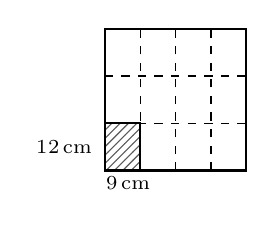
\begin{tikzpicture}[x=1cm, y=1cm, every node/.style={font=\fontsize{7.2pt}{9.2pt}\selectfont, text=black}]
      \fill[pattern=north east lines, pattern color=black!65] (0,0) rectangle (0.45,0.60);
      \draw[black, line width=0.8pt] (0,0) rectangle (1.80,1.80);
      \foreach \i in {1,2,3} {\draw[black, dashed, line width=0.4pt] (\i*0.45,0) -- (\i*0.45,1.80);}
      \foreach \j in {1,2} {\draw[black, dashed, line width=0.4pt] (0,\j*0.60) -- (1.80,\j*0.60);}
      \draw[black, line width=0.7pt] (0,0) rectangle (0.45,0.60);
      \node[anchor=east] at (-0.04,0.30) {$12\unit{cm}$};
      \node at (0.30,-0.16) {$9\unit{cm}$};
    \end{tikzpicture}
  \end{minipage}\\[4pt]
  \tikz\draw[black, dashed, line width=0.5pt] (0,0) -- (18.4cm,0);\\[3pt]
  \fontsize{8.8pt}{12.8pt}\selectfont
  \textbf{ឆ្លុះបញ្ចាំង (\en{EIA Looking-Back})៖} កាត់បំបែកចតុកោណកែងធំជាការេតូចៗ ប្រើ \dotline[1.6cm] រីឯរៀបផ្គុំប័ណ្ណតូចៗបង្កើតជាការេធំ ប្រើ \dotline[1.6cm]!
\end{tcolorbox}

\vfill

% --- E5 Evaluate ---
\secstrip{ផ្នែកទី ៥ \enbf{(E5 - Evaluate)} ៖ ប្រតិបត្តិសំយោគ (ទំ.២៣) សំណួរវិនិច្ឆ័យ \enbf{A--D} និងសំបុត្រចេញ}{រយៈពេល ១០ នាទី}

\begin{tcolorbox}[
  enhanced, sharp corners, colback=white, colframe=black,
  boxrule=0.8pt, boxsep=2.5pt, top=4.5pt, bottom=4.5pt, left=6pt, right=6pt
]
  \textbf{១) ប្រតិបត្តិសំយោគជាក្រុម ៣ នាក់ (សៀវភៅគោល ទំ.២៣)៖} $x$ ជាចំនួនមួយមាន\textbf{លេខពីរខ្ទង់} ។ $58$ ចែកនឹង $x$ នៅសល់សំណល់ $2$ និង $73$ ចែកនឹង $x$ នៅសល់សំណល់ $3$ ហើយ $85$ ចែកនឹង $x$ នៅសល់សំណល់ $1$ ។ រកចំនួន $x$ នោះ ។\\[3pt]
  $\bullet$ ដកសំណល់ចេញ (\cnum{4})៖ $58 - 2 =$ \dotline[0.9cm],\; $73 - 3 =$ \dotline[0.9cm],\; $85 - 1 =$ \dotline[0.9cm] សុទ្ធតែចែកដាច់នឹង $x$\\[3pt]
  $\bullet$ បំបែក៖ $56 = 2^3\times 7$,\; $70 = 2\times 5\times 7$,\; $84 = 2^2\times 3\times 7 \implies \operatorname{PGCD}(56, 70, 84) =$ \ansbox[1.4cm] $\implies x =$ \ansbox[1.4cm]\\[3.5pt]
  \textbf{២) បិទបេសកកម្ម \en{E1}៖} សិស្ស \dotline[1.0cm] ត្រឹមត្រូវ! $\operatorname{PPCM}(6, 8) =$ \ansbox[1.5cm] ។
\end{tcolorbox}

\vspace{4pt}

\begin{tcolorbox}[
  enhanced, sharp corners, colback=white, colframe=black,
  boxrule=0.8pt, boxsep=2.5pt, top=4.5pt, bottom=4.5pt, left=6pt, right=6pt
]
  \textbf{៣) សំណួរវិនិច្ឆ័យ \en{A--D} (គេឱ្យ $A = 2^3 \times 3$ និង $B = 2 \times 3^2 \times 5$ — តើ $\operatorname{PPCM}(A, B)$ ស្មើមួយណា?)៖}\\[3.5pt]
  \textbf{\en{A.}} $2 \times 3 = 6$ \qquad
  \textbf{\en{B.}} $2^3 \times 3^2 = 72$ \qquad
  \textbf{\en{C.}} $2^4 \times 3^3 \times 5 = 2\,160$ \qquad
  \textbf{\en{D.}} $2^3 \times 3^2 \times 5 = 360$\\[4pt]
  \tikz\draw[black, dashed, line width=0.5pt] (0,0) -- (18.4cm,0);\\[3.5pt]
  \textbf{៤) សំបុត្រចេញ ៦០ វិនាទី៖} រកពហុគុណរួមតូចបំផុតនៃ $12$ និង $15$៖ $12 =$ \dotline[1.4cm], $15 =$ \dotline[1.4cm] $\implies \operatorname{PPCM}(12, 15) =$ \ansbox[1.8cm] ។
\end{tcolorbox}

\vfill

% --- Homework ---
\begin{tcolorbox}[
  enhanced, sharp corners, colback=panelgray, colframe=black,
  boxrule=0.95pt, boxsep=2.5pt, top=4pt, bottom=4pt, left=6pt, right=6pt
]
  {\muol\fontsize{9.0pt}{13.0pt}\selectfont កិច្ចការផ្ទះ \enbf{(}សៀវភៅគោល ទំ.២៤ លេខ ៧, លេខ ៩ និង លេខ ១១\enbf{)}}\\[2.5pt]
  \fontsize{8.7pt}{12.6pt}\selectfont
  $\bullet$ \textbf{លេខ ៧៖} រក $\operatorname{PPCM}$ នៃ៖ ក. $81$ និង $225$;\; ខ. $120$ និង $35$;\; គ. $34, 420$ និង $245$;\; ឃ. $70, 21$ និង $28$;\; ង. $512, 18$ និង $20$;\; ច. $88, 220$ និង $528$ ។\\[2pt]
  $\bullet$ \textbf{លេខ ៩៖} រកចំនួន $x$ ដែលតូចជាងគេបំផុត ដោយដឹងថា $\operatorname{PPCM}(6, x) = 24$ ។\\[2pt]
  $\bullet$ \textbf{លេខ ១១៖} នាឡិកាបីរោទ៍រៀងរាល់ $10$ នាទី, $15$ នាទី និង $20$ នាទីម្ដង ។ រករយៈពេលខ្លីបំផុតដែលនាឡិកាទាំងបីរោទ៍ព្រមគ្នាម្ដងទៀត ។
\end{tcolorbox}

% ============================================================================
% ទំព័រទី ៣៖ ទំព័រគ្រូបង្រៀន (គំរូប្លង់ក្ដារខៀន ៣ ផ្នែក + ចម្លើយផ្ទៀងផ្ទាត់រហ័ស)
% ============================================================================
\clearpage
\pagebanner{ទំព័រគ្រូបង្រៀន ៖ ប្លង់ក្ដារខៀន \enbf{(}គ្មាន \enbf{LCD)} និងចម្លើយផ្ទៀងផ្ទាត់រហ័ស}{៦. ពហុគុណរួមតូចបំផុត \en{PPCM} និងសំយោគ (\en{DIV26})}

\secstrip{១. គំរូប្លង់បែងចែកក្ដារខៀន ៣ ផ្នែក សម្រាប់ថ្នាក់រៀនគ្មាន \enbf{LCD}}{សម្រាប់គ្រូប្រើដីស/ហ្វឺត}

\begin{center}
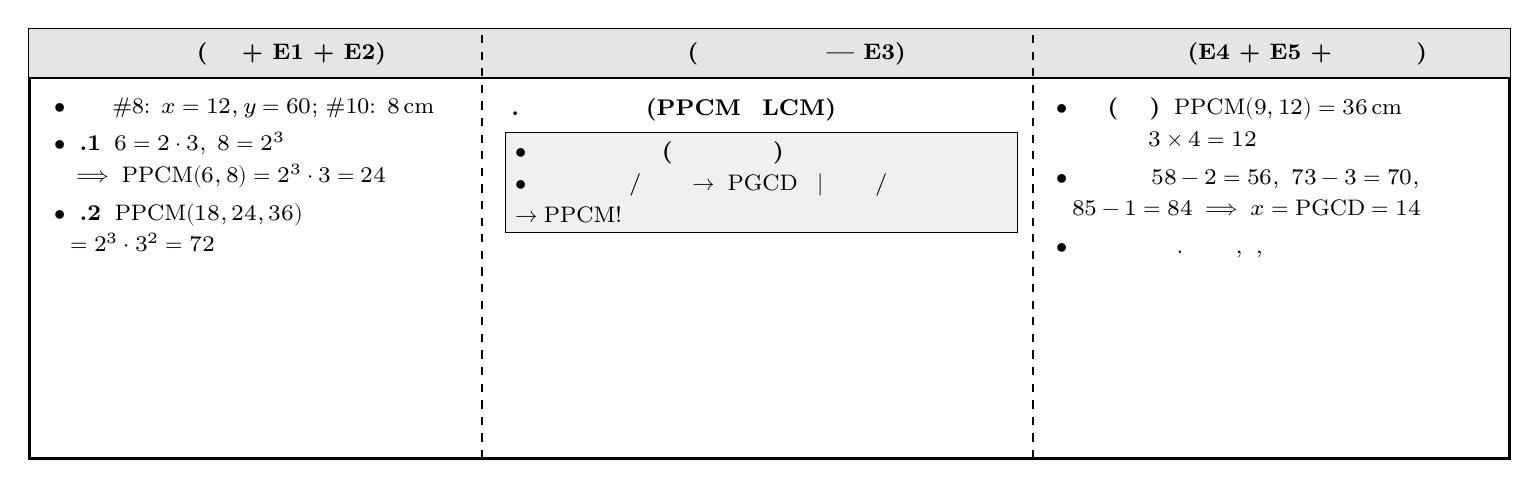
\begin{tikzpicture}[x=1cm, y=1cm, every node/.style={font=\fontsize{8.1pt}{11.5pt}\selectfont, text=black}]
  \draw[black, line width=1.1pt] (0,0) rectangle (18.8,5.45);
  \fill[gray!20] (0,4.83) rectangle (18.8,5.45);
  \draw[black, line width=0.7pt] (0,4.83) -- (18.8,4.83);
  \draw[black, dashed, line width=0.7pt] (5.75,0) -- (5.75,5.45);
  \draw[black, dashed, line width=0.7pt] (12.75,0) -- (12.75,5.45);

  \node at (2.875,5.14) {\textbf{ផ្នែកឆ្វេង (កំណែ + \en{E1} + \en{E2})}};
  \node at (9.25,5.14) {\textbf{ផ្នែកកណ្ដាល (ខ្លឹមសារគោលរក្សាទុក — \en{E3})}};
  \node at (15.775,5.14) {\textbf{ផ្នែកស្ដាំ (\en{E4} + \en{E5} + កិច្ចការផ្ទះ)}};

  % Left
  \node[anchor=north west, text width=5.30cm] at (0.20,4.70) {%
    $\bullet$ \textbf{កំណែ៖} \#8: $x=12, y=60$; \#10: $8\unit{cm}$\\[2pt]
    $\bullet$ \textbf{ឧ.1៖} $6=2\cdot 3,\ 8=2^3$\\
    \hspace*{0.2cm}$\implies \operatorname{PPCM}(6,8) = 2^3\cdot 3 = 24$\\[2pt]
    $\bullet$ \textbf{ឧ.2៖} $\operatorname{PPCM}(18,24,36)$\\
    \hspace*{0.2cm}$= 2^3\cdot 3^2 = 72$
  };

  % Center
  \node[anchor=north west, text width=6.65cm] at (5.92,4.70) {%
    {\muol\fontsize{8.2pt}{11.8pt}\selectfont ៦\enbf{.} ពហុគុណរួមតូចបំផុត \enbf{(PPCM} ឬ \enbf{LCM)}}\\[3pt]
    \tikz\node[draw=black, fill=gray!12, inner sep=3.5pt, text width=6.25cm]{%
      $\bullet$ \textbf{ជាទូទៅ៖} គុណ\textbf{កត្តារួម (និទស្សន្តធំជាងគេ)} ជាមួយនឹង\textbf{កត្តាមិនរួមទាំងអស់} ។\\
      $\bullet$ \textbf{ញែកចំណោទ៖} បំបែក/ចែកស្មើ $\to \operatorname{PGCD}$ $\;\mid\;$ ផ្គុំ/ជួបដំណាលគ្នា $\to \operatorname{PPCM}$!
    };
  };

  % Right
  \node[anchor=north west, text width=5.65cm] at (12.92,4.70) {%
    $\bullet$ \textbf{គំរូ (ប័ណ្ណ)៖} $\operatorname{PPCM}(9,12) = 36\unit{cm}$\\
    \hspace*{0.2cm}ចំនួនប័ណ្ណ៖ $3\times 4 = 12$ សន្លឹក\\[2pt]
    $\bullet$ \textbf{ប្រតិបត្តិ៖} $58-2=56,\ 73-3=70,$\\
    \hspace*{0.2cm}$85-1=84 \implies x = \operatorname{PGCD} = 14$\\[2pt]
    $\bullet$ \textbf{កិច្ចការផ្ទះ៖} ទំ.២៤ លេខ ៧, ៩, ១១
  };
\end{tikzpicture}
\end{center}

\vfill
\secstrip{២. ចម្លើយផ្ទៀងផ្ទាត់រហ័សសម្រាប់សន្លឹកកិច្ចការសិស្ស \enbf{(}ទំព័រ ១ និង ទំព័រ ២\enbf{)}}{\en{Answer Key}}

\begin{tcolorbox}[
  enhanced, sharp corners, colback=white, colframe=black,
  boxrule=0.8pt, boxsep=2.5pt, top=4pt, bottom=4pt, left=6pt, right=6pt
]
  \fontsize{8.8pt}{12.9pt}\selectfont
  $\bullet$ \textbf{ផ្នែក \en{E1}៖} \textbf{សិស្ស ខ} ត្រឹមត្រូវ ($\operatorname{PPCM}(6,8)=24$) ។ \textbf{ផ្នែក \en{E2}៖} \en{E2-A}: $\operatorname{PPCM}(6,8)=\mathbf{24}$; \en{E2-B}: $\operatorname{PPCM}(18,24,36)=\mathbf{72}$, $\operatorname{PGCD}=\mathbf{6}$, $2\times 24=6\times 8=\mathbf{48}$ ។\\[2pt]
  $\bullet$ \textbf{ផ្នែក \en{E4}៖} $9=3^2,\ 12=2^2\times 3 \implies \operatorname{PPCM}=\mathbf{36\unit{cm}}$ ($3\times 4 = \mathbf{12}$ សន្លឹក) ។ \en{EIA}៖ $\operatorname{PGCD}$ ទល់នឹង $\operatorname{PPCM}$ ។\\[2pt]
  $\bullet$ \textbf{ផ្នែក \en{E5}៖} ១) $56, 70, 84 \implies \operatorname{PGCD}=\mathbf{14} \implies \mathbf{x=14}$ ។ ៣) \textbf{ជម្រើស \en{D}} ($360$) ។ ៤) សំបុត្រចេញ៖ $\operatorname{PPCM}(12,15)=\mathbf{60}$ ។
\end{tcolorbox}

\vfill
\secstrip{៣. ចម្លើយលម្អិតនៃកិច្ចការផ្ទះ \enbf{(}សៀវភៅគោល ទំ.២៤ លេខ ៧, លេខ ៩ និង លេខ ១១\enbf{)}}{សៀវភៅគោល ទំ.២៤}

\begin{tcolorbox}[
  enhanced, sharp corners, colback=white, colframe=black,
  boxrule=0.8pt, boxsep=2.5pt, top=4pt, bottom=4pt, left=6pt, right=6pt
]
  \fontsize{8.45pt}{12.4pt}\selectfont
  $\bullet$ \textbf{លេខ ៧៖} ក. $81=3^4,\ 225=3^2\cdot 5^2 \implies 3^4\cdot 5^2=\mathbf{2\,025}$;\; ខ. $120=2^3\cdot 3\cdot 5,\ 35=5\cdot 7 \implies 2^3\cdot 3\cdot 5\cdot 7=\mathbf{840}$;\; គ. $34=2\cdot 17,\ 420=2^2\cdot 3\cdot 5\cdot 7,\ 245=5\cdot 7^2 \implies 2^2\cdot 3\cdot 5\cdot 7^2\cdot 17=\mathbf{49\,980}$;\; ឃ. $70=2\cdot 5\cdot 7,\ 21=3\cdot 7,\ 28=2^2\cdot 7 \implies 2^2\cdot 3\cdot 5\cdot 7=\mathbf{420}$;\; ង. $512=2^9,\ 18=2\cdot 3^2,\ 20=2^2\cdot 5 \implies 2^9\cdot 3^2\cdot 5=\mathbf{23\,040}$;\; ច. $88=2^3\cdot 11,\ 220=2^2\cdot 5\cdot 11,\ 528=2^4\cdot 3\cdot 11 \implies 2^4\cdot 3\cdot 5\cdot 11=\mathbf{2\,640}$ ។\\[2pt]
  $\bullet$ \textbf{លេខ ៩៖} ដោយ $6 = 2\times 3$ និង $\operatorname{PPCM}(6, x) = 24 = 2^3\times 3$ នោះ $x$ ត្រូវតែមានកត្តា $2^3 = 8$ ។ ដើម្បីឱ្យ $x$ តូចបំផុត មិនចាំបាច់មានកត្តា $3$ ឡើយ $\implies \mathbf{x_{\min} = 8}$ ($\operatorname{PPCM}(6,8)=24$ — តម្លៃ $x$ ទាំងអស់ដែលផ្ទៀងផ្ទាត់គឺ $8$ និង $24$) ។\\[2pt]
  $\bullet$ \textbf{លេខ ១១៖} $10=2\cdot 5,\ 15=3\cdot 5,\ 20=2^2\cdot 5 \implies \operatorname{PPCM}(10, 15, 20) = 2^2\cdot 3\cdot 5 = \mathbf{60}$ \textbf{នាទី} ($= \mathbf{1}$ \textbf{ម៉ោង}) ទើបរោទ៍ព្រមគ្នាម្ដងទៀត ។
\end{tcolorbox}

\vfill
\secstrip{៤. ចំណុចប្រុងប្រយ័ត្នគរុកោសល្យ និងកំហុសបោះពុម្ពសៀវភៅគោល \enbf{(}ទំ.២៤ លេខ ៧\enbf{)}}{\en{Pedagogical Watchlist}}

\begin{tcolorbox}[
  enhanced, sharp corners, colback=panelgray, colframe=black,
  boxrule=0.85pt, boxsep=2.5pt, top=4pt, bottom=4pt, left=6pt, right=6pt
]
  \fontsize{8.45pt}{12.4pt}\selectfont
  $\bullet$ \textbf{កំហុសបោះពុម្ពខ្វះសញ្ញាក្បៀសនៅទំ.២៤ លេខ ៧ (គ, ឃ, ង)៖} ក្នុងសៀវភៅគោលបានបោះពុម្ពដកឃ្លាគ្មានក្បៀស៖ «គ. $34\;\; 420$ និង $245$», «ឃ. $70\;\; 21$ និង $28$», «ង. $512\;\; 18$ និង $20$» ។ សូមគ្រូបញ្ជាក់ប្រាប់សិស្សថា ចំណុចនីមួយៗជាការរក $\operatorname{PPCM}$ នៃ\textbf{ចំនួន ៣ តួ} (ដាក់សញ្ញាក្បៀសរវាងតួទី១ និងតួទី២) មិនមែនចំនួនប្រាំខ្ទង់ទេ!
\end{tcolorbox}

\end{document}
